\chapter{Analyse et Spécification des Besoins}

\section*{Introduction du chapitre}
La réussite d'un projet logiciel repose sur une compréhension fine et formalisée des
besoins. Ce chapitre présente la démarche d'analyse adoptée, identifie les acteurs du
système et leurs rôles, puis détaille les besoins fonctionnels et non-fonctionnels de
QuickTriage. Il se conclut par la présentation de la méthodologie de gestion de projet
retenue, accompagnée de sa planification.

\section{Étude des besoins}

\subsection{Méthodologie d'analyse}
L'analyse des besoins a été conduite selon une démarche itérative et centrée utilisateur.
Elle s'est appuyée sur trois leviers : (i) l'étude du domaine métier (fonctionnement du
triage, échelle KTAS, contraintes des urgences) ; (ii) l'analyse des données disponibles
afin de vérifier la faisabilité de la prédiction ; et (iii) la projection des scénarios
d'usage sur le terrain, pour garantir l'adéquation de l'outil aux contraintes réelles du
soignant (rapidité, lisibilité, fiabilité). Les besoins ainsi recueillis ont été classés en
besoins fonctionnels (ce que le système doit faire) et non-fonctionnels (les qualités
attendues).

\subsection{Acteurs du système}
Trois acteurs principaux interagissent avec QuickTriage. Le tableau~\ref{tab:acteurs} en
précise les rôles.

\begin{table}[h]
\centering
\renewcommand{\arraystretch}{1.4}
\begin{tabular}{p{4cm} p{10cm}}
\toprule
\textbf{Acteur} & \textbf{Rôle et responsabilités} \\
\midrule
\textbf{Personnel soignant / Infirmier de tri} & Acteur principal. Saisit les constantes
vitales du patient, déclenche la prédiction, consulte le niveau de priorité proposé et la
confiance associée. Reste le décideur final du triage. \\
\textbf{Médecin} & Valide ou corrige la proposition du système, supervise les cas critiques
et exploite l'information de priorité pour organiser la prise en charge. \\
\textbf{Administrateur} & Gère la configuration technique (déploiement du modèle, version,
paramètres), assure la maintenance et le suivi du bon fonctionnement du système. \\
\bottomrule
\end{tabular}
\caption{Acteurs du système QuickTriage et leurs rôles.}
\label{tab:acteurs}
\end{table}

\begin{infobox}
QuickTriage est explicitement un \textbf{outil d'aide à la décision}. Le niveau KTAS proposé
est une recommandation ; la responsabilité du triage demeure celle du personnel soignant et
du médecin.
\end{infobox}

\section{Besoins fonctionnels}
Les besoins fonctionnels décrivent les services que le système doit rendre. Ils sont
synthétisés dans le tableau~\ref{tab:bf}.

\begin{table}[h]
\centering
\renewcommand{\arraystretch}{1.3}
\begin{tabular}{p{1.6cm} p{4.2cm} p{8cm}}
\toprule
\textbf{Réf.} & \textbf{Besoin} & \textbf{Description} \\
\midrule
BF1 & Saisie des constantes & Permettre la saisie rapide des paramètres vitaux du patient
(âge, état mental, douleur/NRS, SBP, DBP, HR, RR, BT, saturation, mode d'arrivée, etc.). \\
BF2 & Prédiction du niveau KTAS & Calculer automatiquement la classe de priorité
(CRITIQUE / URGENT / NON\_URGENT) à partir des constantes saisies. \\
BF3 & Affichage du résultat & Restituer la classe prédite, le délai maximal associé et le
niveau de confiance, avec un code couleur de priorité. \\
BF4 & Indicateur de criticité & Signaler explicitement les cas critiques
(\texttt{isCritical}) pour attirer l'attention du soignant. \\
BF5 & Détail des probabilités & Afficher la répartition des probabilités entre les trois
classes pour une lecture nuancée. \\
BF6 & Validation clinique & Permettre au soignant/médecin de valider ou corriger la
proposition. \\
BF7 & Historique des triages & Conserver une trace des évaluations réalisées (consultation
ultérieure). \\
BF8 & Gestion de version du modèle & Exposer la version du modèle utilisé
(\texttt{modelVersion}) pour la traçabilité. \\
\bottomrule
\end{tabular}
\caption{Besoins fonctionnels de QuickTriage.}
\label{tab:bf}
\end{table}

\section{Besoins non-fonctionnels}
Les besoins non-fonctionnels expriment les qualités attendues du système. Compte tenu du
domaine médical, ils revêtent une importance particulière.

\begin{table}[h]
\centering
\renewcommand{\arraystretch}{1.3}
\begin{tabular}{p{3.2cm} p{10.6cm}}
\toprule
\textbf{Catégorie} & \textbf{Exigence} \\
\midrule
\textbf{Performance / Latence} & L'inférence doit être quasi instantanée (chargement unique
du modèle ONNX au démarrage, réponse de l'API en deçà de quelques centaines de
millisecondes). \\
\textbf{Fiabilité} & Le système doit fournir des prédictions stables et reproductibles ;
priorité au rappel des cas CRITIQUES pour limiter le sous-triage. \\
\textbf{Sécurité des données} & Les données de santé étant sensibles, l'accès à l'API doit
être protégé, les échanges sécurisés (HTTPS) et la collecte minimisée. \\
\textbf{Utilisabilité} & Interface mobile claire, saisie rapide, lecture immédiate du
résultat grâce au code couleur, adaptée à un usage sous pression. \\
\textbf{Scalabilité} & Architecture capable d'absorber des montées en charge (statelessness
des services EJB, modèle chargé en singleton). \\
\textbf{Maintenabilité} & Code modulaire, séparation nette des couches (ML, backend,
frontend), métadonnées de prétraitement externalisées pour faciliter les mises à jour du
modèle. \\
\textbf{Interopérabilité} & Recours au format ONNX et à une API REST standard pour
découpler l'entraînement du déploiement. \\
\bottomrule
\end{tabular}
\caption{Besoins non-fonctionnels de QuickTriage.}
\label{tab:bnf}
\end{table}

\section{Méthodologie de gestion de projet}

\subsection{Choix et justification}
Compte tenu de la nature exploratoire du volet \textit{data science} (où les résultats
d'une étape conditionnent les choix de la suivante) et du besoin d'itérations fréquentes,
une démarche \textbf{agile et incrémentale} a été retenue. Le projet a été découpé en
incréments livrables, chacun apportant une valeur vérifiable : préparation des données,
modèle de référence, optimisation, intégration backend, application mobile. Cette approche a
notamment permis de réagir rapidement à la découverte de la fuite de données, en
réorientant le projet vers un nouveau jeu de données sans remettre en cause l'ensemble de la
planification.

\subsection{Planification}
La figure~\ref{fig:gantt} présente le diagramme de Gantt synthétisant le déroulement du
projet sur la période considérée. Les grandes phases s'enchaînent tout en autorisant des
recouvrements (par exemple, le début de l'intégration backend pendant l'affinage du
modèle).

\begin{figure}[h]
\centering
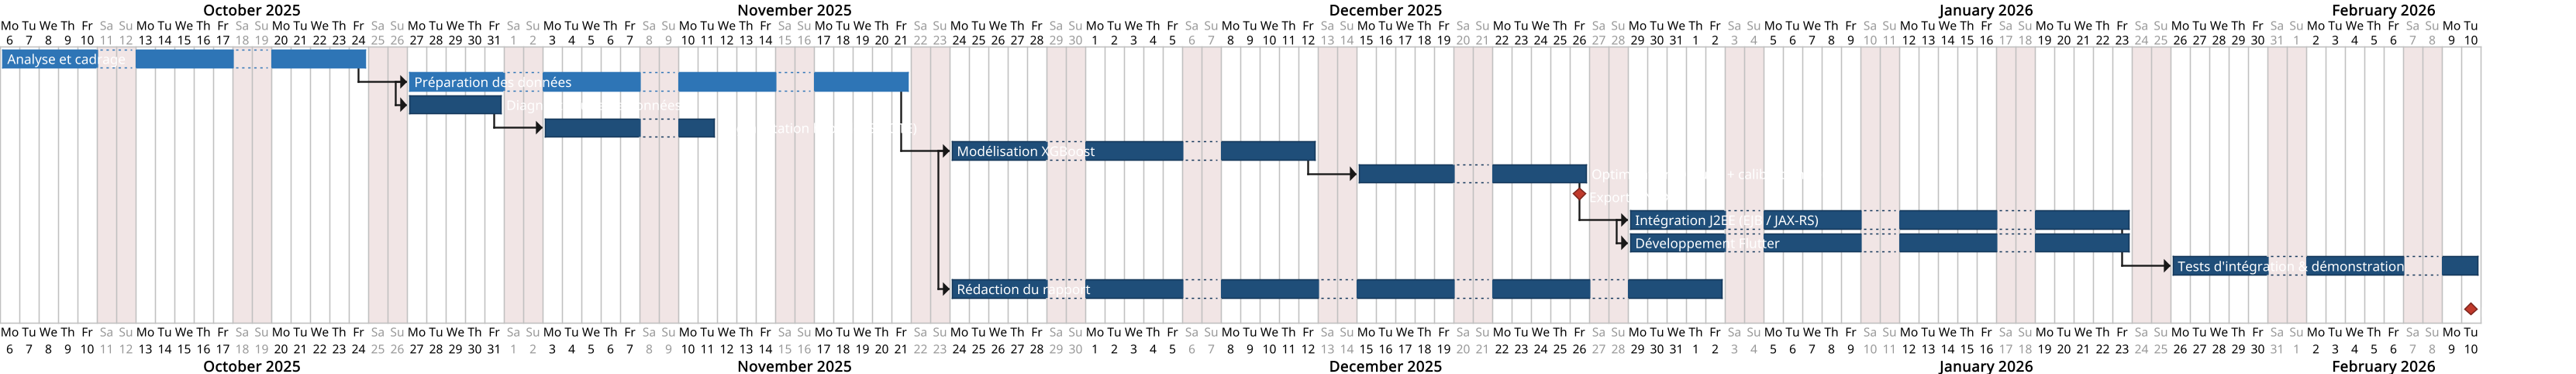
\includegraphics[width=\textwidth]{images/gantt.png}
\caption{Diagramme de Gantt du projet QuickTriage.}
\label{fig:gantt}
\end{figure}

\noindent Les principales phases sont les suivantes :
\begin{enumerate}
  \item \textbf{Analyse et cadrage} : étude du domaine, des échelles de triage et des
  besoins.
  \item \textbf{Préparation des données} : exploration, diagnostic de la fuite de données,
  changement de jeu de données, nettoyage, augmentation hybride.
  \item \textbf{Modélisation} : entraînement du modèle de référence puis du modèle XGBoost.
  \item \textbf{Optimisation et calibration} : recherche d'hyperparamètres avec Optuna,
  calibration du seuil de la classe CRITIQUE.
  \item \textbf{Intégration backend} : export ONNX, chargement du modèle, services EJB, API
  REST JAX-RS.
  \item \textbf{Développement frontend} : application mobile Flutter et consommation de
  l'API.
  \item \textbf{Tests, démonstration et rédaction} : validation de bout en bout et
  documentation.
\end{enumerate}

\section*{Conclusion du chapitre}
Ce chapitre a formalisé les besoins de QuickTriage : identification des acteurs, besoins
fonctionnels et non-fonctionnels, puis méthodologie de gestion de projet et planification.
Ces spécifications constituent le socle sur lequel reposera la conception. Le chapitre
suivant traduit ces besoins en une architecture système cohérente, articulant les couches
machine learning, backend et frontend.
